\documentclass[titlepage]{article}
\usepackage[utf8]{inputenc}
\usepackage{fancyhdr}
\usepackage{titling}
\usepackage{tabto}
\usepackage[ddmmyyyy]{datetime}
\usepackage{graphicx}
\usepackage{listings}
\usepackage{siunitx}
\usepackage[bottom]{footmisc}
\renewcommand{\dateseparator}{.}
\renewcommand{\figurename}{Obr.}
\renewcommand{\contentsname}{Obsah}
\graphicspath{ {/home/andras/Documents/kop/img/} }
\title{\textbf{Jednozvodový elektrokardiograf} \\
\large Praktická časť odbornej zložky maturitnej skúšky}
\date{\empty}

\begin{document}

\bgroup
	\fancypagestyle{empty} {
		\fancyhead[C] {Stredná priemyselná škola elektrotechnická S. A. Jedlika v Nových Zámkoch}
		\fancyfoot[L] {
			\begin{flushleft}
				Nové Zámky, 2019
			\end{flushleft}		
		}
		\fancyfoot[R] {
			\begin{flushright}
				riešiteľ: \textbf{András Zemes} \\
				ročník štúdia: \textbf{štvrtý}
			\end{flushright}
		}
		\fancyfoot[C] {\empty}		
	}
	\maketitle
\egroup


\section*{Praktická časť odbornej zložky maturitnej skúšky}
a \underline{Zadanie úlohy pre komplexnú maturitnú skúšku:} 
\newline

\begin{description}
	\item [Meno a priezvisko:]
		\tabto{4cm} András Zemes
		
    \item [Trieda:]	
    	\tabto{4cm} 4. IT
    	
	\item [Konzultant:]		 	  
		\tabto{4cm} Mgr. Peter Hudec
		
	\item [Školský rok:] 
		\tabto{4cm} 2018/2019
		
	\item [Odbor:]		  
		\tabto{4cm} Informačné a sieťové technológie
		
	\item [Názov témy:]			  
		\tabto{4cm} Jednozvodový elektrokardiograf 
		
	\item [Úloha:]				  
		\tabto{4cm} Zhotoviť prístroj, \emph{elektrokardiograf}, na snímanie 
		\tabto{4cm} a zachytenie elektrických potenciálov srdca.
		
	\item [Špecifikácia úlohy:] \hfill
	
    \begin{enumerate}
		\item Naštudovanie a spracovanie potrebnej teórie
		\begin{itemize}
			\item Elektrický potenciál srdca
        	\item Prehľad prístrojov EKG
        	\item Signál a jeho spracovanie
		\end{itemize}
    	\item Vytvorenie a konštrukcia prístroja na meranie EKG
    	\item Vytvorenie elektronickej časti, práca s mikrokontrolérom
    	\item Vytvorenie PC aplikácie na grafické zobrazenie spracovaných údajov
    	\item Webové rozhranie ku spracovaným dátam
	\end{enumerate}
	
	\item [Praktický charakter úlohy:]
		Návrh plošného spoja, programovanie 
		\tabto{4cm} mikrokontroléra, vytvorenie grafickej aplikácie.
		
\end{description}
	
\vspace{10mm}
\hrulefill
\\\hspace*{0mm}\phantom{v.r.: }András Zemes, riešiteľ

\vspace{10mm}
\hrulefill
\\\hspace*{0mm}\phantom{v.r.: }Mgr. Peter Hudec, interný konzultant

\vspace{10mm}
\hrulefill
\\\hspace*{0mm}\phantom{v.r.: }Zástupkyňa riaditeľa školy

\vspace{10mm}
V Nových Zámkoch dňa \today


\section*{Čestné vyhlásenie}

Ja, dolupodpísaný András Zemes, študent 4. IT triedy Strednej priemyselnej školy S. A. Jedlika v Nových Zámkoch, týmto vyhlasujem, že som túto prácu   vyhotovil sám, s použitím uvedenej literatúry a podľa rád môjho konzultanta. 

\vspace{10mm}
\hrulefill
\\\hspace*{0mm}\phantom{v.r.: }András Zemes
\newpage

\section*{Poďakovanie}
Touto cestou by som sa chcel poďakovať všetkým, ktorí mi akýmkoľvek spôsobom pomohli a povzbudzovali ma pri vypracovaní mojej komplexnej maturitnej práce. Predovšetkým však patrí moja vďaka konzultantovi, Mgr. Petrovi Hudecovi, za jeho všestrannú pomoc, za vedenie a cenné pripomienky pri záverečnom spracovaní práce.

\newpage
\tableofcontents

\newpage
\section{Úvod}
Ľudské telo je zázračný živý organizmus, ktorý sa správa podľa zákonitostí prírody a biológie. Dnes známa podoba Homo sapiens je výsledkom prirodzeného evolučného výberu, ktorým prechádza už dlhé tisícročia. Vďaka nemu sú naše orgány vyspelé a odolné, dokonale slúžia prežitiu. Ich rola a presný spôsob fungovania však dlho zostávali záhadou pred lekármi a vedcami v minulosti. Revolučné objavy a výdobitky v medicíne viedli k podrobnému zmapovaniu a poznaniu ľudského tela, i keď mnoho fenoménov je doposiaľ nevysvetlených. Choroby a nemoci sa stali liečiteľnými a predĺžil sa predpokladaný vek dožitia.

V modernej dobe sa výrazne zmenil štýl, akým žijeme. Jeho dôsledky nesú naše telá, ktoré neboli stavané na rušný, uponáhľaný spôsob života a na zvládanie každodenného stresu. Nesprávna životospráva, zlé návyky a degradácia životného prostredia majú záporny vplyv na zdravotný stav obyvateľstva a prispievajú k šíreniu civilizačných ochorení. Jedná sa o degeneratívne ochorenia, ktoré patria medzi najpálčivejšie globálne zdravotnícke problémy. V rebríčkoch najčastejších príčin smrti sa často vyskytujú na prvých miestach.

Škodlivé zvyklosti ako nezdravé stravovanie, nadváha, nedostatok fyzickej aktivity, fajčenie a nadmerná konzumácia alkoholu sa odzrkadľujú aj na srdci a obehovej sústave. Tieto a mnoho ďalších faktorov zvyšujú riziko srdcovocievnych ochorení vrátane kôrnatenia tepien, infarktu myokardu, vysokého krvného tlaku, atď. Ľudia si veľakrát ani neuvedomujú, že sa u nich vyvíja takáto choroba alebo si to uvedomia neskoro.

Riešenie môže poskytnúť bioinformatika a biomedicínske inžinierstvo. Sú to vedné disciplíny, ktoré sa zaoberajú zhromažďovaním a vyhodnocovaním biologických dát a konštrukciou klinických zariadení. Vo veľkej miere uľahčujú prácu lekárom vo včasnom rozpoznaní a liečbe zdravotných problémov. Klasickým príkladom biomedicínskeho prístroja je elektrokardiograf alebo v skratke EKG. 

V roku 1903 Willem Einthoven zostrojil prvý funkčný elektrokardiograf. Použil strunový galvanometer na snímanie elektrických potenciálov z končatín pacienta. Jeho vynález sa stal základným kameňom elektrokardiografie, za ktorý neskôr získal Nobelovu cenu za fyziológiu alebo medicínu. Vďaka Einthovenovi lekári dostali prvýkrát v histórii možnosť nahliadnuť hlboko do srdca a odhaliť skryté defekty prevodového systému.

Myslím si, že najväčším nepriateľom ľudstva je neinformovanosť. Pokiaľ chceme predísť chorobám a žiť zdravý, plnohodnotný život, musíme poznať možné následky rizikového správania. Zámerom tejto práce je šíriť povedomie o dôležitosti starania sa o zdravie a preukázať, že pozorovanie vnútrotelových javov nemusí byť tak zložité ako sa na prvý pohľad zdá. 



\newpage
\section{Ciele}
Kľúč úspešného elektrotechnického projektu spočíva v dokonalej spolupráci jeho elektronických a informačných zložiek. Zámerom tejto práce je poukázať na to, že aj pomerne jednoduchými komponentmi sa dajú vyriešiť komplexné problémy. 

Dôležité aspekty výslednej práce sú univerzálnosť, portabilita a intuitívny dizajn. Prístroj by mal dokázať použiť každý bez špeciálneho vybavenia a bez podrobnej znalosti jeho fungovania. Riešenie má byť taktiež prenosné, aby bolo neobmedzene využiteľné.

Pri návrhu plošného spoja sa muselo prihliadať i na bezpečnosť pri použití prístroja. Elektrokardiograf sleduje pulz snímaním elektrických potenciálov srdca z povrchu tela elektródami. Napájaním obvodu batériami a ochranou malým napätím sa zabránilo výskytu nečakaných a potenciálne rizikových situácií.

Pomocou jednozvodového EKG vieme určiť pulz, srdcový rytmus, ba aj odhaliť prítomnosť srdových arytmií a fibrilácie predsiení. Projekt môže taktiež slúžiť ako pomôcka pri výučbe elektroniky, programovania či informatiky. Znázorňuje fungovanie signálových filtrov, operačných zosilňovačov, mikrokontrolérov a grafických počítačových aplikácií.

\newpage
\section{Teória elektrokardiografie}
\subsection{Elektrofyziológia srdca}

Základom vnútorného fungovania srdca je jeho elektrická aktivita. Srdce je jedinečný orgán z hľadiska, že jeho elektrická činnosť nie je nervovo založená. Vykonávajú ju špecializované vodivé svalové bunky. Zväzky takýchto buniek podmieňujú čerpaciu schopnosť srdca.

Svalové kontrakcie sú riadené elektrickými impulzmi, ktoré sa šíria po prevodovom systéme a pracovnom myokarde. Menia elektrické potenciály na rôznych bodoch pokožky približne o tisícinu voltu (1 mV). Táto elektrická aktivita skrýva v sebe neuveriteľné množstvo informácií, prostredníctvom ktorých získame náhľad do fungovania tohto zázračného orgánu.

Zdrojom týchto impulzov je sinoatriálny (SA) uzol, ktorý sa nachádza v stene hornej časti pravej predsiene. Udáva frekvenciu kontrakcií myokardu (srdcového svalstva), ktorá je nominálne 70 tepov za minútu.

Signály sa ďalej šíria vodivými dráhami predsiení a stimulujú svalové kontrakcie. Pokračujú po srdcovej priehradke, septe, ktorá oddeľuje dve polovice srdca. Blízko bodu spojenia štyroch dutín srdca sa nachádza zhluk špeciálnych buniek - atrioventrikulárny (AV) uzol. Uzol AV postup vzruchov mierne inhibuje a následne ich vysiela do Hisovho zväzku.

Hisov zväzok  sa delí na dve vetvy, tzv. Tawarove ramienka. Obidve vetvy vedú do siete Purkyňových vláken, ktoré aktivujú pracovný myokard.
\\
\\

\begin{figure}[!ht]
\begin{center}
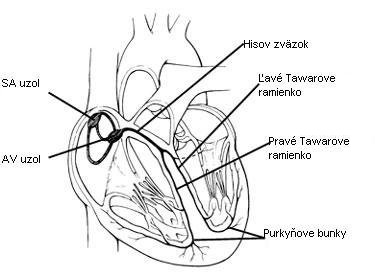
\includegraphics[scale=0.7]{48_img1_b}
\caption{Prevodový systém srdca}
\end{center}
\end{figure}

\newpage
\subsection{Akčný potenciál}
Ako vyrába a prenáša srdcové tkanivo elektrické impulzy? Aby sme si priebeh tohto deja mohli vysvetliť, musíme sa preniesť až na úroveň atómov.

\emph{Atóm je neutrálny,} ak má rovnaký počet protónov (kladne nabitých častíc) a elektrónov (záporne nabitých častíc). 

\emph{Ióny vznikajú} z elektricky neutrálnych atómov pridaním resp. ubraním elektrónov. 

V pokoji je srdcová bunka v \emph{polarizovanom stave}:
\begin{itemize}
	\item mimobunkový priestor je elektricky pozitívny pre vysokú koncentráciu kladných iónov sodíka a vápnika
	\item vnútrobunkový priestor je oproti vonkajšej strane negatívny
	\item rozdiel potenciálov je -90mV
\end{itemize}

Keď pokojový membránový potenciál dosiahne určitú prahovú hodnotu (cca. 15 mV), tzv. \emph{akčný potenciál}, tento pokojový stav sa náhle zmení. V membráne bunky sa otvoria prieduchy a kladne nabité ióny prúdia späť do bunky. Táto náhla strata polarizácie sa volá depolarizácia a vzniká pri nej elektrický prúd.

Po depolarizácii nastáva protikladný dej, repolarizácia, keď sa ióny znovu prečerpávajú von mimo membránu. Depolarizačná vlna vyvolávaná uzlom SA sa šíri po prevodovom systéme srdca a uvádza svaly do pohybu. Proces, ktorý začal pumpovaním iónov takto končí pumpovaním krvi. 

\begin{figure}[!ht]
\begin{center}
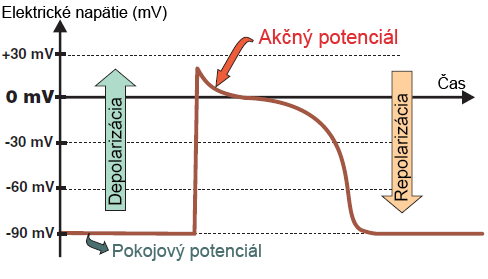
\includegraphics[scale=0.5]{action-potential-voltage}
\caption{Akčný potenciál v grafickom vyobrazení}
\end{center}
\end{figure}

%https://www.jfmed.uniba.sk/fileadmin/jlf/Pracoviska/ustav-patologickej-fyziologie/07Pregradualne_studium/01Vseobecne_lekarstvo/04Handouty_a_prednasky/01Handouty/01Elektrokardiografi1-jun10.pdf


\newpage 
\subsection{Prehľad prístrojov EKG}
\subsubsection{Druhy funkčných vyšetrení}
Elektrokardiografia je jedným zo základných lekárskych vyšetrení. Najčastejšie sa využíva v núdzových situáciách pri podozrení na srdcový infarkt, na zistenie poruchy súvisiacej s kardiovaskulárnym systémom alebo ako preventívne vyšetrenie so zámerom odhaliť možný srdcový defekt.

Vyšetrenie EKG je neinvazívne a nevyžaduje žiadnu špeciálnu prípravu. Pri klasickom EKG sa elektródy pripevnia na hrudník, zápästia a členky pacienta. Elektrické signály zachytené z povrchu tela, ktoré sú spravidla veľmi slabé, v rádoch milivoltov, prístroj zosilní a zaznamená. Následne ich lekár vyhodnotí.

Existuje niekoľko rôznych druhov vyšetrní:
\subsubsection*{Štandardné 12-zvodové EKG}
Je najčastejšie používaný zo všetkých typov EKG. Pozostáva zo 6 končatinových zvodov a 6 hrudných zvodov. Každý zvod je samostatne zapisovaný na priebežne sa posunujúci špeciálny záznamový papier, prípadne zobrazuje hodnoty na monitore.
\subsubsection*{Záťažové EKG (ergometria)}
Ukáže správanie srdca a obehového systému pri námahovej aktivite. Na simuláciu sa väčšinou používa stacionárny bicykel alebo bežecký pás. Monitoruje sa záznam EKG v súvislosti s krvným tlakom. Na zázname sa pátra po zmenách, ktoré na EKG urobenom v pokoji nie sú viditeľné.
\subsubsection*{Dynamické EKG}
Umožňuje sledovať srdcovú činnosť pri bežných aktivitách počas 12-48 hodín. Zvýšením doby monitorovania sa zvyšuje pravdepodobnosť nálezu nepravidelností rytmu alebo námahových ischémií myokardu v zázname.
\subsubsection*{Tlakový Holter}
Ambulantné 24-hodinové sledovanie krvného tlaku je jednoduché vyšetrenie často indikované pri diagnostikovaní hypertenzie. Sníma sa tlak krvi v domácom prostredí pri každodenných činnostiach pomocou nafukovacej manžety.
\\
\\
EKG určuje základné fyziologické hodnoty ako sú frekvencia srdcovej činnosti, rytmus, elektrická os srdca, prevodové časy a morfológia segmentov EKG krivky. Na základe týchto parametrov môže byť stanovená diagnóza a rozpoznaná porucha srdcového rytmu (arytmia), porucha prevodu elektrických vzruchov, ischemická choroba srdca a iné patologické zmeny v myokarde.


\newpage


\subsubsection{Časti klasického prístroja EKG}

\textbf{Tepelná tlačová hlava}
\\
Kreslí EKG krivku generovaním tepla.
\\
\\
\textbf{Termopapier}
\\
Prichádza do kontaktu s tlačovou hlavou. Na mieste dotyku sa farba papiera mení na čiernu, takto vzniká krivka EKG. Papier je tiež citlivý na tlak.
\\
\\
\textbf{Elektródy}
\\
Elektródy sú vyrobené z vodivého materiálu, ktorý dokáže zachytiť elektrické impulzy zo srdca. Signály odosielajú na spracovanie do meracieho prístroja cez pripojené káble.
\\
\\
\textbf{Zosilňovač}
\\
Zosilňovač je zariadenie, ktoré sa nachádza v elektrokardiografe a zvyšuje amplitúdu elektrického signálu. Signály prichádzajúce zo srdca sú relatívne slabé (0,0001V až 0,003V) a je potrebné ich zosilniť.
\\
\\
\textbf{Galvanometer}
\\
Premieňa prúd na mechanický pohyb.
\\
\\
\textbf{Sada EKG káblov}
\\
Slúžia na spojenie zvyčajne desiatich elektród s hlavnou jednotkou prístroja EKG. Takáto konfigurácia umožňuje monitorovať srdce z 12 ,,pohľadov".

\subsubsection{Výdobytky modernej elektrokardiografie}
Moderné prístroje EKG disponujú zabudovanými mikroprocesormi, ktoré ich riadia a rozširujú ich diagnostické schopnosti. Vďaka sofistikovaným matematickým algoritmom a modelom sú schopné previesť zložitú analýzu signálu a automaticky ho vyhodnotiť. Sú kompaktné, prenosné a vhodné i na monitorovanie mimo zdravotníckeho zariadenia.

Prepojiteľnosť s počítačom je v dnešnej dobe takmer samozrejmosťou, niektoré dokonca komunikujú bezdrôtovo a aj na diaľku. Digitalizácia údajov môže byť výhodná naporíklad z hľadiska archivácie alebo v prípade potreby zdieľať záznam so špecialistom.

Kardiologický monitor je častým rozšírením zariadenia EKG a umožňuje dlhodobo sledovať srdcovú aktivitu pacienta. Údaje zobrazuje v reálnom čase a ponúka náhľad kriviek ešte pred ich zápisom na papier.


\newpage

\subsection{Umiestnenie elektród}
Tri končatinové elektródy (pravá ruka, ľavá ruka, ľavá noha)  vytvárajú Einthovenov trojuholník. Vzniknú 3 \emph{bipolárne zvody} reprezentované stranami trojuholníka. Každý zvod pozostáva z dvoch elektród, z pozitívneho a z negatívneho. Pozitívny a negatívny pól spolu tvoria elektrický vektor, ktorý sa premieta na papier.

\begin{description}
	\item Zvod I: \tabto{1cm} $V_{I} = \phi_L - \phi_R$
	\item Zvod II: \tabto{1cm} $V_{II} = \phi_F - \phi_R$
	\item Zvod III:	\tabto{1cm} $V_{III} = \phi_F - \phi_L$
\end{description}
, kde: \\
\tabto{1cm} $V_{I}$ = napätie zvodu I\\
\tabto{1cm} $V_{II}$ = napätie zvodu II\\
\tabto{1cm} $V_{III}$ = napätie zvodu III\\
\tabto{1cm} $\phi_L$ = potenciál na ľavej ruke\\
\tabto{1cm} $\phi_R$ = potenciál na pravej ruke\\
\tabto{1cm} $\phi_F$ = potenciál na ľavej nohe\\
\\
Podľa Kirchhoffovho zákona platí, že veľkosť potenciálov (amplitúd na EKG zázname) v zvode $V_{II}$ je sumou potenciálov v zvodoch $V_{I}$ a  $V_{III}$:
\tabto{1cm} $V_{I} + V_{III} = V_{II}$
, z čoho vyplýva, že iba dva z troch zvodov sú nezávislé.
\\
\\
Einthoven definoval rozdiely potenciálov medzi troma pármi horeuvedených bodov ako základné končatinové zvody v elektrokardiografii.


\begin{figure}[!ht]
\begin{center}
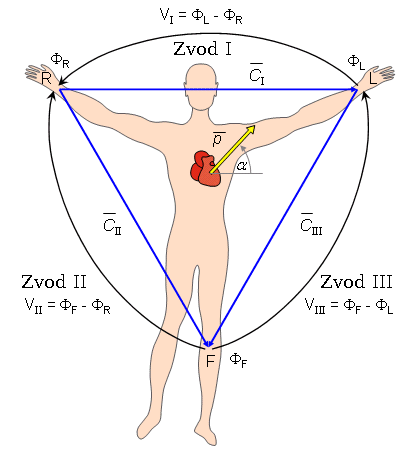
\includegraphics[scale=0.4]{ekg-zvody}
\caption{Einthovenove končatinové zvody a Einthovenov trojuholník}
\end{center}
\end{figure}
%http://www.bem.fi/book/15/15.htm


\subsection{Signál a jeho spracovanie}
Po úspešnom zmeraní a zosilnení signálu čelíme zložitej prekážke v snahe zachytiť srdcový rytmus. Signál je síce zosilnený, ale naďalej obsahuje mnoho nežiaducich elementov vplyvom rušivých faktorov z okolia. Výsledkom je skreslený biosignál, ktorý je v tejto fáze nepoužiteľný.

Nepresnosti v meraniach odborne nazývame \emph{artefakty}. Artefakty sa môžu prejavovať v menšej či väčšej miere v závislosti od nedokonalostí v priebehu vedenia signálu z pacienta do aparatúry (prístroja). V elektrokardiografii rozoznávame tri základné druhy artefaktov:
\begin{itemize}
	\item sieťový brum
	\item kolísanie nulovej línie (drift)
	\item myopotenciály
\end{itemize}

V minimalizácii nežiaduceho šumu nám napomáha súbor špecializovaných hardvérových i digitálnych filtrov.

\subsubsection{Sieťový brum}
Prvým krokom spracovania signálu je základná hardvérová filtrácia. Elektromagnetická interferencia (EMI) vzniká pôsobením  elektromagnetického poľa z elektrickej siete. Pri tomto jave dochádza k vzniku indukovaného napätia (Ui) a indukovaného prúdu na vodiči. Šum opísaného druhu môžeme charakterizovať pri frekvencii 50 Hz sínusového rušenia. Na potlačenie sieťového brumu je účinná kombinácia hardvérového RC článku s digitálnym filtrom. 

\subsubsection{Potlačenie driftu}
Drift alebo kolísanie nulovej línie opisuje skupinu elektrochemických a mechanických javov. Príkladmi elektrochemických sú potenie pod elektródami, nedostatočné odmastenie pokožky, malé množstvo kontaktného gélu. Dýchanie (do 0,8 Hz) a pomalé pohyby klienta (do 2 Hz) sú mechanické javy. Na odstránenie nízkofrekvenčnej rušivej zložky použijeme hornopriepustný filter.

\subsubsection{Myopotenciály}
Ďalší rušivý faktor pri vyšetrení EKG predstavuje svalová aktivita, najmä pri záťažovom EKG. Svaly počas pohybu vytvárajú elektrické impulzy, ktoré sa potom prejavujú vo forme muskuloskeletálneho artefaktu. Najväčším problémom v zdolaní účinku myopotenciálov je vzájomné prekrývanie frekvenčného pásma svalovej aktivity a užitočného pásma EKG. Na odstránenie tohto artefaktu nie je účinná pásmová priepusť. Vyžaduje sa pokročilejšie riešenie, napríklad pomocou adaptívnej filtrácie. 

\newpage
\subsubsection{Voľba filtrov}
\subsubsection*{Nekonečná impulzná odozva - IIR}
\subsubsection*{Konečná impulzná odozva - FIR}



\begin{figure}[!ht]
\begin{center}
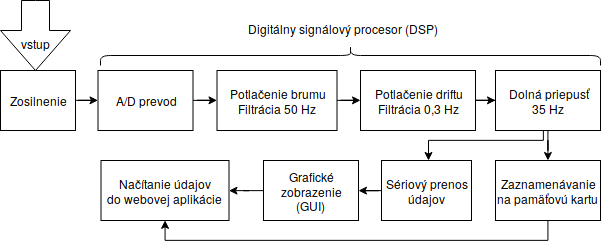
\includegraphics[scale=0.4]{flowchart}
\caption{Bloková schéma spracovania EKG}
\end{center}
\end{figure}

\newpage
\section{Metodika práce}
\subsection{Návrh a konštrukcia hardvéru}
Proces návrhu hardvérových komponentov som si rozdelil do niekoľkých fáz kvôli systematickosti. Takýto spôsob práce mi umožnil priebežné testovanie a odhaľovanie možných chýb počas vývoja. Od začiatku až po finálny dizajn som prešiel tromi iteráciami projektu. 

Na návrh elektroniky a dizajn plošných spojov som používal grafický počítačový editor Eagle (verzia 9.1.3).

\subsubsection{Zosilňovací obvod na vývojovej doske}
Prvý prototyp obvodu bol vyrobený podľa jednoduchej schémy. Pozostávala iba z jedného operačného zosilňovača a zopár rezistorov. Z bezpečnostných dôvodov bola namiesto laboratórneho zdroja použitá 9V batéria na napájanie obvodu. 

Operačný zosilňovač LM741 slúži na zosilnenie nízkonapäťového vstupu z elektród priložených na povrch tela. Je zapojený v diferenčnej konfigurácií, jeho invertujúci a neinvertujúci vstup predstavujú rozdielne napätia. Výstup je teda funkciou napäťovej diferencie medzi dvoma hrudnými elektródami. Faktor zisku je približne 50 podľa pomeru R5:R4. Z dôvodu, že zosilňovač funguje optimálne pre stredové hodnoty (medzi maximom a minimom), je nutné jeho vstupy dostať do použiteľného pásma. Na tento účel slúži napäťový delič R1-R2.

Analógový výstup bol pripojený do 3,5 mm mikrofónového rozhrania zvukovej karty počítača. Signál prešiel základnou softvérovou filtráciou a bol graficky zobrazovaný pomocou počítačovej aplikácie.

Hlavnou problematikou tohto návrhu bola všeobecná nespoľahlivosť a výskyt elektromagnetickej interferencie a iných artefaktov v meraných hodnotách.


\begin{figure}[!ht]
\begin{center}
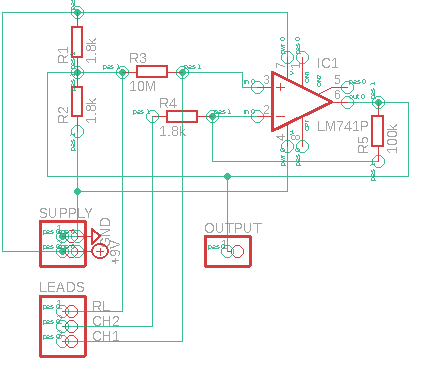
\includegraphics[scale=.9]{schematic}
\caption{Schéma zosilňovacieho obvodu}
\end{center}
\end{figure}

\newpage
\subsubsection{Spájkovaný obvod}
Ďalším krokom bolo navrhnúť plošný spoj v Eagli podľa vyššej uvedenej schémy zosilňovacieho obvodu. Na základe počítačového návrhu bol zhotovený druhý prototyp na spájkovateľnej vývojovej doske. Elektrické súčiastky boli osadené a pospájané vodivými cestami z cínu. Doska mala celkovo 6 vývodov:
\begin{itemize}
	\item VCC (+5V) napájanie
	\item GND - zem
	\item OUT - analógový výstup
	\item Hrudný zvod č. 1
	\item Hrudný zvod č. 2
	\item Pravá noha
\end{itemize}
Signál bol meraný a spracúvaný za pomoci Arduina UNO. Výstup zo zosilňovača bol spojený s analógovým pinom Arduina A0 (ADC). Vykresľovanie krivky EKG sa zrealizoval zabudovaným nástrojom programu Arduino IDE, ktorý sa nazýva Serial Plotter.

Zobrazovaný signál bol do veľkej miery znečistený, preto bolo nutné použiť softvérový filter. Najjednoduchší filter vhodný na úlohu bol súčasťou oficiálnej knižnice Filters.h. \footnote{Dokumentácia a zdrojové kódy k spomínanej knižnici sú dostupné na webovom sídle \textit{https://playground.arduino.cc/Code/Filters}}

Nasledovný kód je implementáciou dolnopripustného filtra RC, ktorý slúži na vyhladenie signálu. Filter je nastavený na frekvenciu 50 Hz. Obsahuje deklaráciu premenných a inicializáciu triedy FilterOnePole.

\begin{lstlisting}
float filterFrequency = 5.0; 

FilterOnePole lowpassFilter(LOWPASS, filterFrequency);

while(true) {
  lowpassFilter.input(analogRead(INPUT_PIN));
}
\end{lstlisting}

Filter funguje na báze nekonečnej impulznej odozvy (IIR). Hlavnou výhodou je, že riešenie kladie veľmi nízke nároky na pamäť a výpočtovú kapacitu. Veľké pozitívum znamená taktiež jednoduchosť implementácie do projektu. Onedlho sa však prejavili seriózne problémy spôsobené vlastnosťami spomínaného filtra. Po úvodnom zachytení impulzov amplitúda postupne klesala, až kým nedosiahla nulu. Takéto správanie je nepriaznivým vedľajším účinkom IIR filtrov. 

\newpage
\subsubsection{Finálny obvod a rozširovacie moduly}
Výsledný produkt zahŕňa niekoľko dôležitých komponentov. Ústrednú časť štruktúry zariadenia tvorí osobitne navrhnutý a na mieru vyrobený plošný spoj. Táto doska priamo spája analógovú časť aplikácie dovedna s digitálnym signálovým procesorom. Ďalej je doplnená o dva rozširovacie moduly a batérie.

\subsubsection*{Mikroprocesor}
Mikroprocesor je centrálnym prvkom zariadenia. Zodpovedá za digitalizáciu a spracúvanie príchodzieho signálu, riadenie a koordináciu jednotlivých elektrických článkov v rámci aplikácie a odovzdávaie informácii počítaču.

Pri výbere mikroprocesora sa prihliadalo na výkon, úspornosť, počet vývodov a na veľkosť dostupnej programovej pamäte. Nakoniec sa uprednostnil 8-bitový mikroradič Atmega328P z rodiny megaAVR od firmy Atmel. Vyhovel všetkým požiadavkám projektu, je vhodný na úlohu DSP a disponuje kvalitnou dokumentáciou i komunitnou podporou zo strany vývojárov. 
Podrobnosti o mikroprocesore sú opísané v tabuľke nižšie.\footnote{Informácie boli čerpané zo stránky výrobcu \textit{www.microchip.com/wwwproducts/en/ATmega328p}}

\begin{table}[htb]
\begin{tabular}{ll}
\textbf{Parameter}              & \textbf{Hodnota}     \\
Typ programovej pamäte          & Flash                \\
Veľkosť programovej pamäte (KB) & 32                   \\
Max. rýchlosť CPU (MIPS)        & 20                   \\
Komunikačné periférie           & 1-UART, 2-SPI, 1-I2C \\
Tepelná tolerancia (C)          & -40 do 85            \\
Napájacie napätie (V)           & 1,8 do 5,5           \\
Počet vývodov                   & 28                  
\end{tabular}
\end{table}

\subsubsection*{Napaľovanie zavádzača}
Zavádzač (angl. bootloader) mikroprocesora je prvý program, ktorý sa spustí pri každom štarte. Asistuje pri nahrávaní kódu do flash pamäte a čip sa stáva samoprogramovacím, čím zaniká potreba programátora.

Samostatný čip Atmega328P sa dodáva bez zavádzača, tým pádom sa priamo nedá programovať. Proces napaľovania bootloadera riadi medzičlánok zvaný in-system program (ISP). Na túto rolu vyhovuje aj doska Arduino UNO.

Prvým krokom je nahrať šablónu ArduinoISP na dosku. Potom sa prepojí mikročip s Arduinom podľa špecifickej schémy zapojenia. V nastaveniach sa zvolí typ dosky ,,Arduino Duemilanove alebo Nano" pre 16 MHz konfiguráciu. Za programátor sa vyberie možnosť ,,Arduino as ISP".

Po dôkladnej kontrole všetkých nastavení sa môže spustiť nahrávanie zavádzača (Tools $\rightarrow$ Burn Bootloader).


\newpage
\subsubsection*{FT232RL programátor s Mini USB}
Adaptér USB–serial zabezpečuje programovanie čipov a komunikáciu s nimi. Komunikácia prebieha cez UART, tj. cez Rx a Tx piny. Úspešné nahratie programu má jednu podmienku: na čipe sa musí nachádzať zavádzač. Modul je kompatibilný s napätiami 3.3V a taktiež 5V, ladenie sa umožňuje pomocou prepínača. Zapojenie musí byť doplnené o kondenzátor (\SI{0,1}{\micro\F}) a o pull up rezistor na vývode DTR, aby resetovanie mohlo správne prebehnúť.

\begin{table}[htb]
\begin{tabular}{ll}
\textbf{FT232RL}  	& \textbf{Atmega328}   \\
DTR          		& RESET                \\
TXD			 		& RX                   \\
RXD					& TX				   \\
5V					& VCC				   \\
CTS (clear to send) & patrí do štandardu FT232, nie je nutné ho použiť \\
GND					& GND
\end{tabular}
\end{table}

\subsubsection*{Slot pre Micro SD kartu}
Slot umožňuje čítanie a zapisovanie údajov na Micro SD kartu. Prenos údajov sa uskutočňuje cez štandardné SPI rozhranie. Modul funguje s logickým napätím 3.3V, avšak vďaka zabudovaného regulátora toleruje aj 5V. Tým pádom je plne kompatibilný so všetkými Arduino doskami a s príslušnou natívnou knižnicou \emph{SD.h} z ponuky Arduino IDE.

\subsubsection*{Výroba integrovaného plošného spoja}
Hotový digitálny návrh skompletizovaného plošného spoja bol odoslaný do výroby profesionálnemu výrobcovi. K objednávke bol priložený súbor \textit{.brd} vyexportovaný z projektu Eagle (viď. prílohu). Špecifikácie objednanej dosky: \\
\emph{Jednostranný plošný spoj so spájkovateľným ochranným lakom} \\
\textbf{Hrúbka dosky a medenej vrstvy:} 1.5 mm, \SI{35}{\micro\m} \\
\textbf{Rozmery PCB:} 65x50 mm \\
\textbf{Počet otvorov:} 87 ks \\

Po doručení objednanej dosky nasledovalo manuálne osadenie súčiastok. Ako prvé boli prispájkované pätice integrovaných obvodov: DIP28 pre mikroprocesor a DIP8 pre operačný zosilňovač. Použitie pätíc sa odporúča v prípade citlivých komponentov z dôvodu, aby sa predišlo ich možnému poškodeniu pri vysokých teplotách počas spájkovania.

Ďalej boli postupne osadené ostatné súčiastky ako kryštál 16 MHz, cievka, rezistory a keramické kondenzátory. Pri osadzovaní bipolárnych súčiastok (napr. svetelné diódy, elektrolytické kondenzátory) sa nesmie zabúdať na správne smerovanie kladných, resp. záporných pólov.

Naposledy boli prispájkované napájacie a vstupnovýstupné piny pre rozširovacie moduly a elektródové vodiče.

\newpage
\subsubsection{Konštrukcia zariadenia}
Posledným krokom v práci s hradvérom bolo umiestniť všetký komponenty do škatuľky. Na tento účel padla voľba na univerzálny kryt HM-1553DGY\footnote{Technický výkres krytu so špecifikáciami a rozmermi sa nachádza na stránke distribútora https://www.tme.eu/sk/Document/bd6787db93f837d8972974413558d5cd/HM-1553DBK.pdf} od Hammmondu s rozmermi 89x147x24 mm v tmavosivom prevedení. Výrobný materiál je plast ABS. Kryt sa skladá z troch častí: z predného panelu a z vrchnej a spodnej časti, ktoré sa uzatvárajú štyrmi skrutkami. 

Napájacie puzdro na tri AA batérie bolo uložené pozdĺžne v zadnej časti krytu. K nemu bol pripevnený zvisle polohovaný USB—Serial modul. Na zadnej stene bol taktiež vytvorený otvor na rozhranie Micro USB.

Okraje hlavného plošného spoja boli upravené a tvarované tak, aby sa doska mohla prichytiť o jeden z podporných stĺpikov. Následne bola vyvŕtaná diera pre svetelnú diódu a vytvorený obdĺžnikový otvor pre vypínač. Na prednom paneli boli vyvŕtané diery s väčším priemerom na vsadenie troch laboratórnych konektorov.

Nakoniec boli všetky komponenty upevnené obojstrannou lepiacou páskou. Rozširovacie moduly, vypínač a konektory boli zapojené do riadiacej dosky či už priamo alebo prepojovacími káblami. Prepojovacie káble museli byť vyrobené na mieru kvôli nevšedným požiadavkám na dĺžku a počet vodičov a tvar prípojky.


\begin{figure}[!ht]
\begin{center}
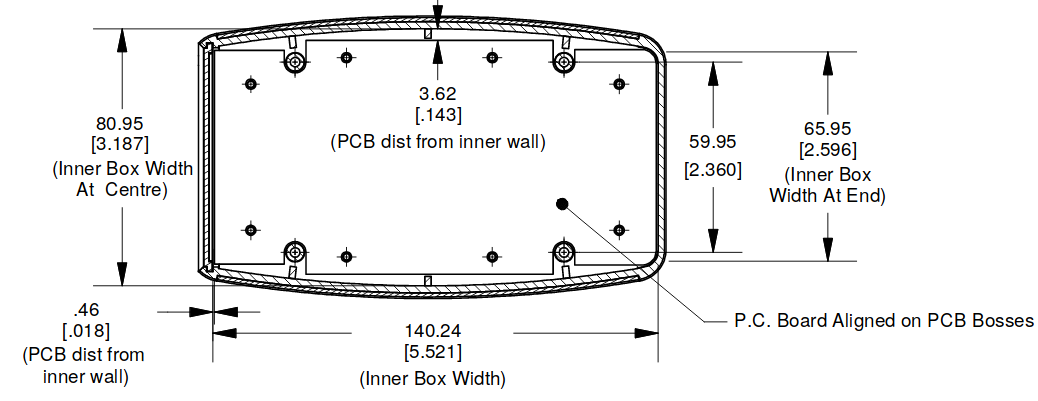
\includegraphics[scale=.3]{assembly-2}
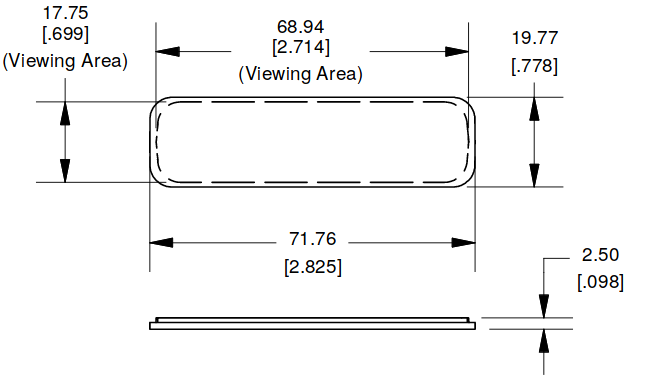
\includegraphics[scale=.3]{assembly-1}
\caption{Nárys a pôdorys škatuľky s rozmermi}
\end{center}
\end{figure}


\newpage
\section*{Zoznam použitej literatúry}
\begin{itemize}
\item GEMINI, spol. s.r.o. 1991. Ľudské telo - Komplexný sprievodca po ľudskom tele a jeho funkciách. Bratislava. ISBN 80-85265-12-5.
\item IAIZZO, Paul A. 2005. Handbook of Cardiac Anatomy, Physiology, and Devices. New Jersey. Human Press, Inc. ISBN 1-59259-835-8.
\item HANÁČEK, Ján, PLEVKOVÁ, Jana. 2009. Elektrokardiografia - Základné mechanizmy porúch elektrickej funkcie srdca a ich manifestácia na Ekg krivke. Martin. Ústav patologickej fyziológie JLF UK.
\item MALMIVUO, Jaakko, PLONSEY, Robert. 1995. Bioelectromagnetism - Principles and Applications of Bioelectric and Biomagnetic Fields. Oxford. Oxford University Press.
\item BÓRIKOVÁ, Ivana. 2016. Funkčné vyšetrenie respiračného, kardiovaskulárneho a močového systému. Portál Jesseniovej lekárskej fakulty Univerzity Komenského. ISSN 1337-7396.
\item MIŠČÍK, Peter. 2011. Zpracování elektrokardiogramu. Vysoké učení technické v Brně. 
\item www.kardiolog.sk/o-srdci/
\item www.techmed.sk/akcny-potencial/
\item www.wikiskripta.eu/w/Rušení\_biosignálů\_a\_artefakty
\item www.swharden.com/wp/2016-08-08-diy-ecg-with-1-op-amp/
\item www.arduino.cc/en/Tutorial/ArduinoToBreadboard
\item www.microchip.com/wwwproducts/en/ATmega328p
\item techfun.sk/produkt/ft232rl-programator-s-mini-usb-5v-3-3v/
\item techfun.sk/produkt/slot-pre-micro-sd-kartu/
\item github.com/tttapa/Filters

\end{itemize}


\end{document}